\documentclass{article}
\usepackage[breakable]{tcolorbox}
\usepackage{amsmath}
\usepackage{pgfplots}
\pgfplotsset{compat=1.17}

\begin{document}

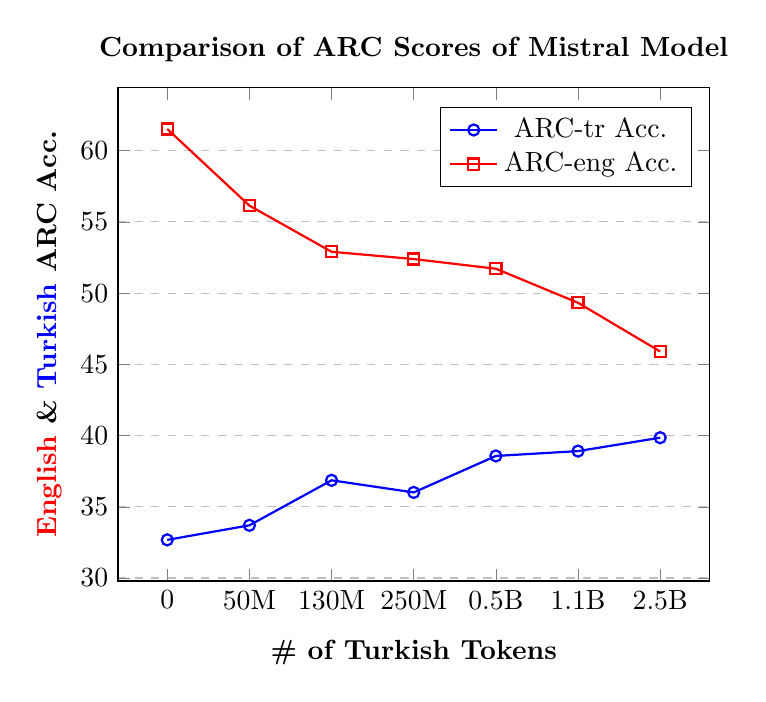
\begin{tikzpicture}
\begin{axis}[
    title={\textbf{Comparison of ARC Scores of Mistral Model}},
    xlabel={\textbf{\# of Turkish Tokens}},
    ylabel={\textbf{\textcolor{red}{English} \&  \textcolor{blue}{Turkish} ARC Acc.}},
    xtick={0,1,2,3,4,5,6},
    xticklabels={
        0,
        50M,
        130M,
        250M,
        0.5B,
        1.1B,
        2.5B,
    },
    xlabel style={at={(0.5,-0.10)}},
    legend pos=outer north east,
    ymajorgrids=true,
    grid style=dashed,
    legend style={cells={align=left}},
    width=0.75\textwidth,
    xtick distance=5,
    legend style={at={(0.97,0.88)},anchor=east},
]

% Adding data for Turkish ARC
\addplot[
    color=blue,
    mark=o,
    thick,
    nodes near coords,
    point meta=explicit symbolic,
] coordinates {
    (0,32.68)
    (1,33.70)
    (2,36.86)
    (3,36.01)
    (4,38.57)
    (5,38.91)
    (6,39.85)
};

% Adding data for English ARC
\addplot[
    color=red,
    mark=square,
    thick,
    nodes near coords,
    point meta=explicit symbolic,
] coordinates {
    (0,61.52)
    (1,56.14)
    (2,52.90)
    (3,52.39)
    (4,51.71)
    (5,49.32)
    (6,45.90)
};

\legend{ARC-tr Acc., ARC-eng Acc.}
\end{axis}
\end{tikzpicture}

\end{document}